\begin{center}
\textit{by P. Bokan, E. Petit, N. Readioff, M. Wielers}
%\textit{Editor E. Petit, ATLAS authorlist in preparation.}
\end{center}

The results presented in Section~\ref{sec:HH_ATLAS} were extended to provide estimates of the prospects at the HE-LHC, assuming a centre of mass collision energy of 27~$\UTeV$ and 15~$\iab$ of data.

The assumption is made that the detector performance will be the same as of the HL-LHC ATLAS detector. Comparisons between simulation at centre of mass energy of 14 and 27~$\UTeV$ show that the kinematic of the Higgs boson decay particles, as well as the $m_{HH}$ distribution are similar. However the pseudorapidity of the particle tends to point more frequently in the forward region, which would decrease the acceptance by around 10\%. This effect is not taken into account and the impact is expected to be small.

The event yields for the various background processes are scaled by the luminosity increase and the cross-section ratio between the two centre of mass energies. For the signal the cross-section of 139.9 fb is used~\cite{Grazzini:2018bsd}.

Without including systematic uncertainties a significance of 7.1 and 10.7 standard deviations is expected for the $b\bar{b}\gamma\gamma$ and $b\bar{b}\tau\tau$ channels respectively.
The hypothesis of no Higgs self-coupling can be excluded with a significance of 2.3 and 5.8 standard deviations respectively. Finally the $\kappa_{lambda}$ parameter is expected to be measured with a 68\% CI precision of 40\% and 20\% respectively.
With the $b\bar{b}\gamma\gamma$ channel, if the HL-LHC systematic uncertainties were considered this precision would be 50\%, dominated by the uncertainty on the photon energy resolution. If this uncertainty were divided by a factor 2 then the precision would be 45\%.



\subsubsection{Comparison of results}

The results presented in Sections~\ref{sec:HH_HE_theory} and \ref{sec:HH_HE_atlas} appear to be quite different, with the $\kappa_{\lambda}$ parameter being measured with a precision of 15\% and 40\% respectively at 68\% CL.
Thoroughful studies were performed to understand the difference. The result from the ATLAS experiment is an extrapolation of the HL-LHC results (which consider a mean pile-up rate of 200) which were optimised to increase the sensitivity to the SM signal, but could be improved for a precise measurement of $\kappa_{\lambda}$. In particular low values of the di-Higgs invariant mass below 400~\GeV\ are suppressed where most of the sensitivity lies.
Using a similar selection as the study of D. Gon\c{c}alves \textit{et al}, 40\% more background events are found using the ATLAS simulation. Half of it comes from missing background processes, while the other half comes from differences in the selection because of the effect of pile-up in the ATLAS simulation.
There is also a categorisation based on the pT-ordering of the jets and b-jets which improves the results as shown in Figure~\ref{fig:bound1} but is hard to reproduce when large pile-up is considered.


In order to get an estimate of the best sensitivity achievable with HE-LHC data, a simple combination of the results of the $b\bar{b}\gamma\gamma$ channel presented in Section~\ref{sec:HH_HE_theory} and the results presented with the $b\bar{b}\tau\tau$ presented in Section~\ref{sec:HH_HE_atlas} is performed. No correlations are taken into account in this combination, and no systematic uncertainties are considered. A precision of around 10\% could be then achieved. The $b\bar{b}\tau\tau$ measurement alone is used as an upper value of this precision, so at this point we can consider that the $\kappa_{\lambda}$ parameter could be measuremed with a precision of 10 to 20\%, as illustrated in Figure~\ref{fig:HH_HELHC_comb}. It should also be noted that the second minimum of the likelihood would be unambiguously excluded at the HE-LHC.

It should be emphasized that these results rely on assumptions of experimental performance in very high pile up environment O(800-100) that would require further validation with more detailed studies, and that no systematic uncertainties are considered at this point. On the other hand these studies do not include the additional decay channels that have already been studied for HL-LHC, and of others that could become relevant at the HE-LHC. Exclusive production modes are also very interesting to take into consideration for this measurement. The potential improvements from these have not yet been assessed yet.


\begin{figure}[!htb]
\centering 
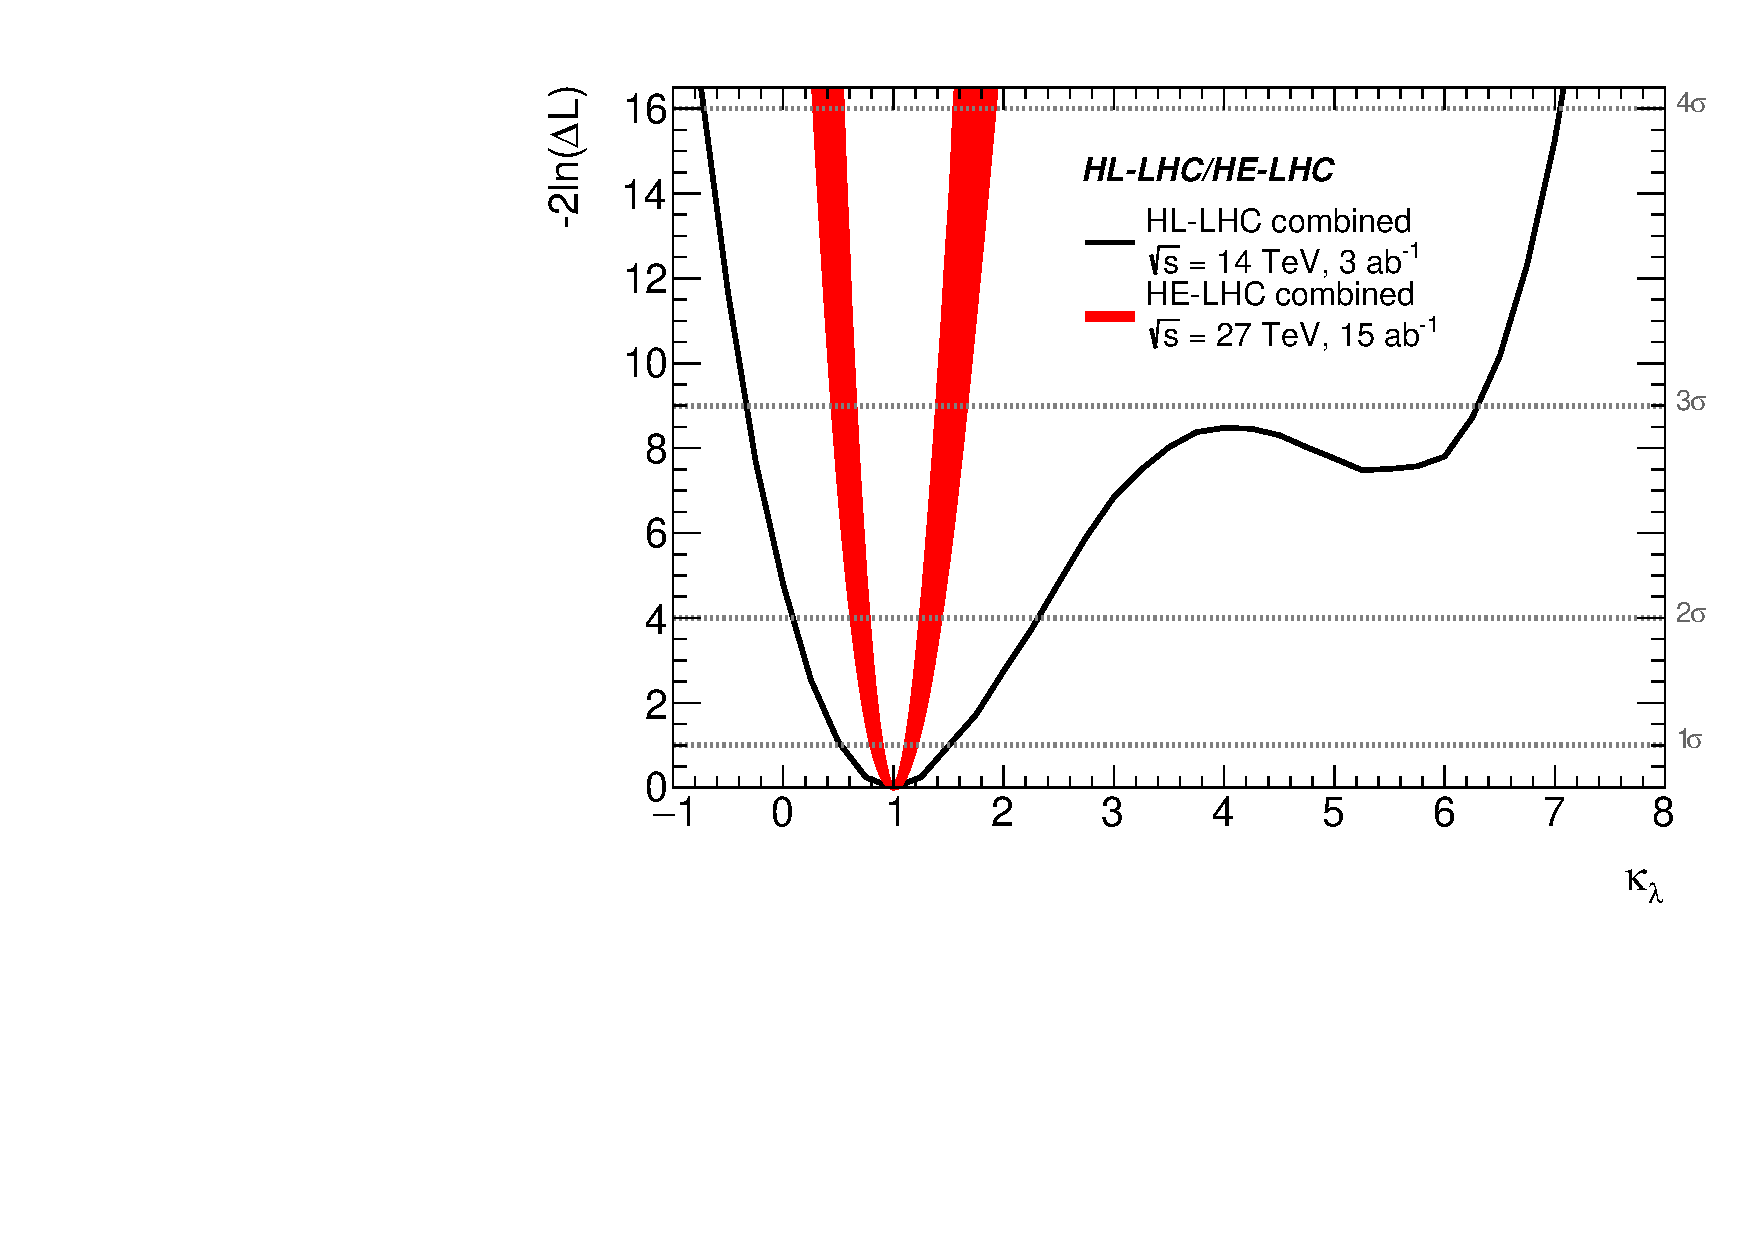
\includegraphics[width=0.7\textwidth]{\main/section3/plots/HELHC_likelihood.pdf}
\caption{Expected sensitivity for the measurement of the Higgs trilinear coupling through the measurement of direct HH production at HE-LHC. The black line corresponds to the combination of ATLAS and CMS measurements with HL-LHC data presented in Section~\ref{sec:HH_Combination}, with systematic uncertainties considered. The red band corresponds to an estimate of the sensitivity using a combination of the $b\bar{b}\gamma\gamma$ and $b\bar{b}\tau\tau$ channels, without systematic uncertainties considered.} 
\label{fig:HH_HELHC_comb} 
\end{figure}
